\parttitle{VII}{End-to-End Forecasting Pipelines}

\section{One pipeline, three tasks}
\label{sec:pipeline-spec}

The three application tasks of Part~VI differ in physics but not in shape:
every competent forecasting study, quantum or classical, traverses the same
nine stages, and this part specifies them once so that the task walkthroughs
of Section~\ref{sec:walkthroughs} can be read as three instantiations of one
object rather than three recipes. The stages, with the discipline attached to
each: \emph{(1)~acquisition} --- source, licence, version pinned
(Table~\ref{tab:datasets}); real versus surrogate declared in every caption
downstream. \emph{(2)~quality control} --- gaps located and \emph{masked, not
filled} unless the fill is itself validated; outages longer than the
autocorrelation time split the series rather than bridging it.
\emph{(3)~target transform} --- forecast the variable the physics makes
stationary ($k_t$, not GHI; anomaly, not SST; residual-after-calendar, not
raw load), because every baseline and error metric inherits this choice.
\emph{(4)~encoding} --- scale inputs to the encoding's natural domain
($[0,1]$ for state replacement, angle range for rotations) using
\emph{training-set} statistics only; choose scalar re-upload, multi-channel
rotations, or state replacement per Part~III. \emph{(5)~reservoir} --- fix
architecture, size, and operating point ($J\Delta t$, Section~\ref{sec:temporal-edge})
before touching test data; record the seed. \emph{(6)~read-out} ---
ridge with $\lambda$ chosen on a chronological validation block or by GCV
(Section~\ref{sec:ridge}); features standardised by training statistics.
\emph{(7)~uncertainty} --- at minimum, residual-quantile intervals; for
operational credibility, pinball-loss quantile read-outs
(Section~\ref{sec:uncertainty}). \emph{(8)~baselines} --- the full Part~I
battery (mean, persistence, linear lags, size-matched ESN) plus the Haar
control; a missing baseline is a missing result. \emph{(9)~interpretation} ---
error decomposed by regime (clear/cloudy, weekday/weekend, event/quiet), not
just averaged; claims scoped to what was actually run.

\begin{table*}[h]
\centering\small
\caption{Where each pipeline stage lives in the shipped code, per framework
path. Stages 1--3 and 6--9 are classical and shared; the framework choice
affects only stages 4--5 (and how features are estimated).}
\label{tab:stage-map}
\begin{tabular}{@{}lp{3.4cm}p{3.2cm}p{3.2cm}p{3.0cm}@{}}
\toprule
Stage & Reference (NumPy) & Cirq & Qiskit & PennyLane \\
\midrule
1--3 data & \multicolumn{4}{l}{\code{datasets.py} (generators and ENSO loader), \code{eda.py} (QC statistics)} \\
4 encoding & \code{input\_state}, $u\!\in\![0,1]$ & $R_Y(\gamma g_i u)$ re-upload & $R_Y$ re-upload, transpiled & broadcast $R_Y$ window \\
5 reservoir & \code{QuantumReservoir} (exact $\rho$) & frozen brickwork, exact $\ev{O}$ & noisy backend, shots, MCM & frozen \code{StronglyEntangling}\newline\code{Layers} block \\
6 read-out & \multicolumn{4}{l}{ridge via \code{ridge\_fit} / GCV variant (Listing~\ref{lst:qiskit}); identical maths in all paths} \\
7--9 & \multicolumn{4}{l}{\code{experiments.py} (baselines, regime slicing, figures); conventions of Part~I} \\
\bottomrule
\end{tabular}
\end{table*}

\section{Reference experiments}
\label{sec:reference-experiments}

All experiments below run the exact reference reservoir
(Section~\ref{sec:reference-impl}) at the shipped configuration --- $n=5$
qubits, $V=4$ virtual nodes, disordered Ising couplings $J=1$, field $h=1$,
seed $7$, thirty features --- with every baseline evaluated at the same feature
count. Everything is \emph{simulation}; solar and load data are
\emph{surrogates}; ENSO is \emph{real}. The scripts print every number quoted.

\subsection{Choosing the operating point: the temporal edge}
\label{sec:temporal-edge}

The one reservoir hyperparameter with no classical analogue intuition is the
injection interval $\Delta t$: how much unitary scrambling the register
undergoes between inputs. Figure~\ref{fig:temporal-edge} sweeps
$J\Delta t$ over $2.5$ decades on NARMA-10. The dependence is strongly
non-monotonic: at $J\Delta t \le 0.25$ the propagator is near identity, the
virtual-node features are nearly collinear, and the model cannot beat the
mean predictor (NMSE $\approx 1.05$); performance improves steeply to a
minimum of $0.283$ at $J\Delta t = 1$; beyond it, over-scrambling degrades
the features to a saturation plateau around $0.6$--$0.75$ for
$J\Delta t \ge 4$. This is the \emph{temporal} edge of
\citet{kobayashi2026edge} reproduced in a five-qubit Ising register: their
analysis identifies two independent optima --- a parametric edge, where the
Hamiltonian sits near the boundary between regular and chaotic level
statistics, and a temporal one, where information injected per step is
scrambled enough to mix into the register but not so much that it
thermalises before read-out --- and prescribes exactly this sweep as the
design procedure. Two practice notes. The optimum is task- and
input-scaling-dependent (Section~\ref{sec:edge-of-chaos}): re-sweep when
either changes. And on hardware the sweep is cheap relative to everything
else, because it reuses the same circuits with a rescaled evolution time ---
there is no excuse for publishing at an arbitrary $\Delta t$.

\begin{figure*}[t]
\centering
\begin{minipage}{0.48\textwidth}
  \centering
  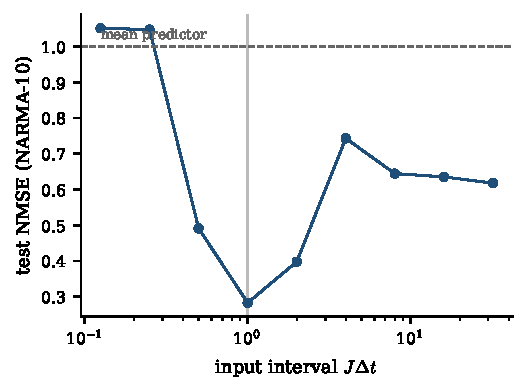
\includegraphics[width=0.98\linewidth]{figures/temporal_edge.pdf}
  \caption{Test NMSE on NARMA-10 versus injection interval $J\Delta t$
  (exact simulation; log axis). The minimum at $J\Delta t=1$ is the temporal
  edge; the dashed line is the mean predictor.}
  \label{fig:temporal-edge}
\end{minipage}\hfill
\begin{minipage}{0.48\textwidth}
  \centering
  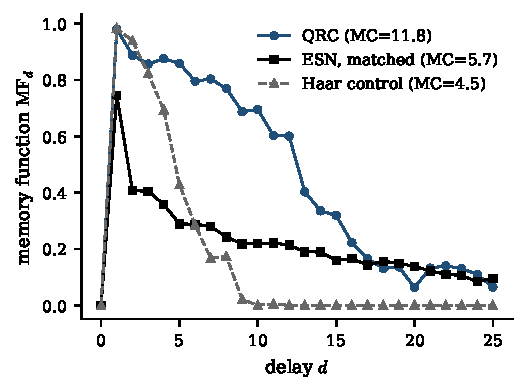
\includegraphics[width=0.98\linewidth]{figures/memory_capacity.pdf}
  \caption{Memory function $\mathrm{MF}_d$ versus delay for the QRC at its
  operating point, the size-matched ESN, and the Haar-random control
  (exact simulation, i.i.d.\ input).}
  \label{fig:memory-capacity}
\end{minipage}
\end{figure*}

\subsection{Memory capacity}
\label{sec:mc-experiment}

At the chosen operating point, Figure~\ref{fig:memory-capacity} shows the
delay-resolved memory function (Eq.~\eqref{eq:mc}, delays to $25$). Total
capacities: QRC $11.8$; size-matched ESN $5.7$; Haar-random control $4.5$.
Two honest readings. First, the \emph{structured} reservoir at its edge
retains linearly recoverable input over roughly twice the delay range of
either control --- and the gap to the \emph{Haar} control specifically shows
this is a property of the tuned dynamics, not of ``being quantum'': a random
unitary of the same size, same observables, same read-out remembers less
than half as much. Second, MC is a diagnostic, not a score: it is measured
on i.i.d.\ input, weights all delays equally, and says nothing about
nonlinearity; the NARMA-10 column below, not this figure, is the performance
claim.

\subsection{Task demonstrations}
\label{sec:task-demos}

Figure~\ref{fig:prediction-demos} shows test-span trajectories for the three
tasks; Table~\ref{tab:results-master} is the complete score sheet.

\begin{figure*}[t]
\centering
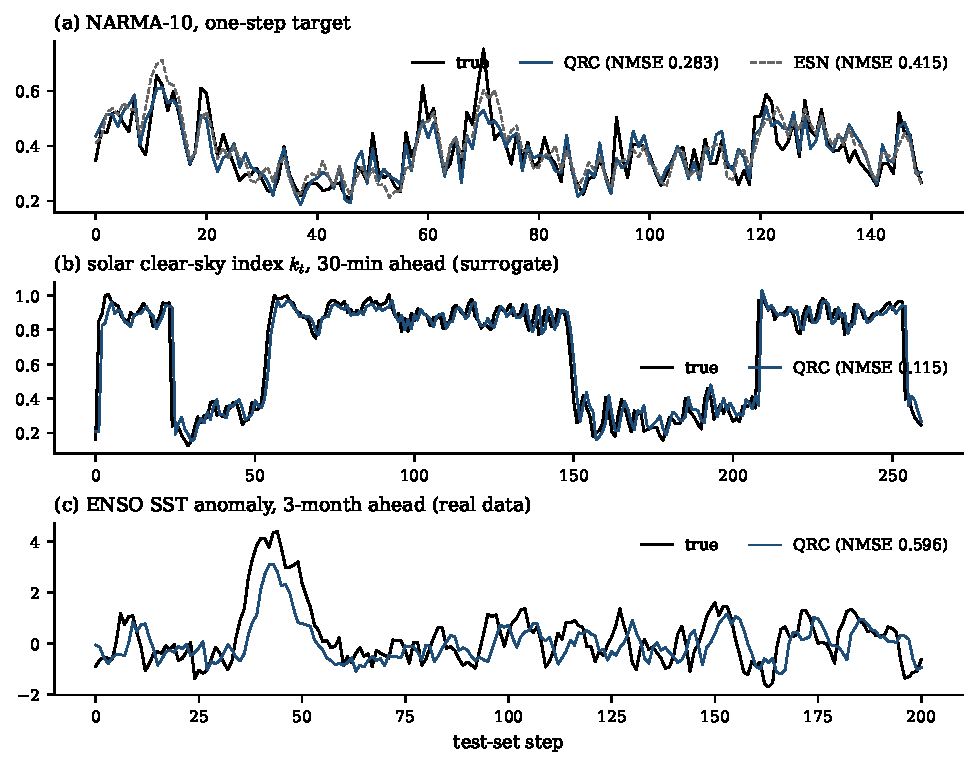
\includegraphics[width=0.92\textwidth]{figures/prediction_demos.pdf}
\caption{Test-span predictions (exact simulation of the reservoir).
(a)~NARMA-10 with QRC and size-matched ESN overlaid; (b)~solar clear-sky
index one step ahead (surrogate data); (c)~ENSO SST anomaly three months
ahead (real data). NMSE values in the legends match
Table~\ref{tab:results-master}.}
\label{fig:prediction-demos}
\end{figure*}

\begin{table*}[t]
\centering\small
\caption{Master results table: test NMSE, exact-expectation simulation,
thirty features for all feature-based models, chronological splits. Bold
marks the best model per task. ``---'' = not applicable.}
\label{tab:results-master}
\begin{tabular}{@{}lccc@{}}
\toprule
Model & NARMA-10 & Solar $k_t$, 1 step (surrogate) & ENSO anomaly, 3 mo (real) \\
\midrule
QRC (Ising, edge) & \textbf{0.283} & 0.115 & 0.596 \\
ESN, size-matched & 0.415 & 0.116 & \textbf{0.555} \\
Haar control & 0.872 & --- & --- \\
Linear lags & 0.740 & \textbf{0.113} & 0.567 \\
Persistence & --- & 0.120 & 0.690 \\
Mean predictor & 1.000 & 1.000 & 1.000 \\
\bottomrule
\end{tabular}
\end{table*}

Reading the table with Part~VIII's eyes. \emph{NARMA-10}: the QRC beats the
size-matched ESN by $32\%$ and the Haar control by $3\times$ --- the designed
benchmark result, on the synthetic task built to reward
memory-plus-nonlinearity, consistent with the small-register literature
\citep{fujii2017harnessing,kutvonen2020optimizing}. \emph{Solar, one step}:
four models within $\pm3\%$ of each other and of persistence --- a statistical
tie. The honest conclusion is that 30-minute-ahead $k_t$ at this site
carries almost no exploitable nonlinear structure beyond its last value, and
\emph{no method}, quantum or classical, adds value here; a study reporting
only the QRC column would look publishable and would mislead.
\emph{ENSO, three months}: every reservoir beats persistence decisively
(memory helps), the tuned ESN leads, and the QRC trails it by $7\%$ --- a
genuinely informative defeat, in two ways. It quantifies the cost of the
window-free but small quantum register on a long-memory task, and against
Part~IV's windowed quantum map on the identical task ($0.747$) it isolates
\emph{recurrence itself} as worth $20$ points of NMSE --- the architectural
conclusion this document considers its most transferable.

\subsection{The shot budget}
\label{sec:shot-budget}

Figure~\ref{fig:shot-noise} replays the NARMA-10 task with the exact
features replaced by finite-shot estimates (eight noise seeds per point).
The analytic ceiling is $0.283$; the sampled model reaches $0.90$ at
$S=10^2$, $0.64$ at $10^3$, $0.53$ at $10^4$, and $0.45$ at $10^5$ ---
converging as $S^{-1/2}$ but still $60\%$ above ceiling at a hundred
thousand shots per feature. The arithmetic this implies for hardware is the
useful output: at thirty features and, say, $S=10^4$, one time step of the
restart protocol costs $3\times10^5$ measured circuits (times the window
length), so a two-thousand-step training series is a $10^9$-shot
commitment --- weeks of queued device time at current throughputs, for a task
a laptop solves exactly in seconds. This is not an argument against hardware
experiments; it is the argument for \emph{small} $T$, batched jobs
(Part~IV), shot-efficient observables, and for treating the eigentask
analysis of \citet{hu2023tackling} and shot-optimal training of
\citet{ahmed2025optimal} as required reading before any device campaign.

\begin{figure*}[t]
\centering
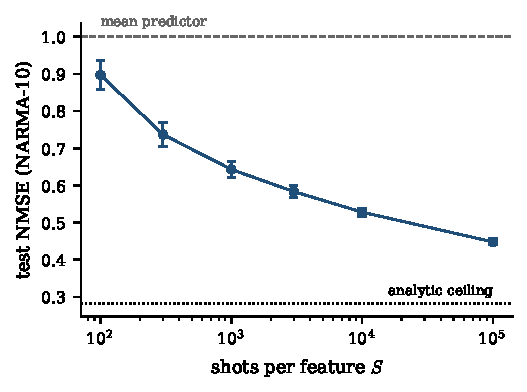
\includegraphics[width=0.5\textwidth]{figures/shot_noise.pdf}
\caption{Shot-noise study on NARMA-10: test NMSE versus shots per feature
$S$ (mean $\pm$ s.d.\ over eight sampling seeds), against the exact-feature
ceiling (dotted) and the mean predictor (dashed). Simulation.}
\label{fig:shot-noise}
\end{figure*}

\section{Task walkthroughs}
\label{sec:walkthroughs}

\subsection{Solar: 30-minute clear-sky index}
\label{sec:pipeline-solar}

\emph{Stages 1--3.} Surrogate NSRDB-like series (real deployment: NSRDB site
extraction, or SURFRAD for minute-scale work); gaps masked ($1.6\%$, longest
$5.5$\,h --- split, never bridge); target $k_t$ per Eq.~\eqref{eq:kt},
daytime only (elevation $>5^\circ$), so the diurnal cycle never inflates
skill. \emph{Stage 4.} Scalar $k_t$, clipped to $[0,1.2]$ then affinely
mapped to $[0,1]$ by training-set range, state-replacement encoding.
\emph{Stage 5.} Reference reservoir at $J\Delta t = 1$. \emph{Stage 6.}
Ridge, $\lambda$ by validation block within the training year.
\emph{Stage 7.} Residual quantiles by cloud regime. \emph{Stage 8--9.}
Table~\ref{tab:results-master}: statistical tie with persistence --- reported
as such. Where a quantum study of this task could still earn its keep, per
the EDA: not the one-step average, but ramp events (regime transitions) and
$2$--$6$\,h horizons where persistence collapses; that is a different target
(Stage~3) and a harder benchmark (event-based scores,
Section~\ref{sec:uncertainty}), and it is listed as research direction R7 in
Part~VIII.

\subsection{Load: day-ahead hourly demand (specified design)}
\label{sec:pipeline-load}

This pipeline is \emph{specified} against the surrogate's EDA but not run in
\code{experiments.py}; it is included because its structure --- the hybrid
posture --- is the one most applications should copy, and it is the natural
first project for a reader (Part~VIII, R6). \emph{Stages 1--3.} GEFCom-like
hourly load with coincident temperature (real deployment: GEFCom2014 load
track, ENTSO-E, or OPSD); target is the residual after a classical
calendar model (hour-of-week means, holiday factor), because
Figure~\ref{fig:eda-load} shows the calendar explains most variance and no
quantum resource should be spent relearning a lookup table.
\emph{Stage 4.} Multi-channel rotation encoding: residual lag, temperature,
CDD --- three channels onto five qubits with fixed random gains.
\emph{Stage 5.} Reference reservoir; re-sweep $J\Delta t$ (the residual's
autocorrelation differs from NARMA's). \emph{Stage 6.} Hybrid read-out:
quantum features concatenated with the calendar prediction and lags ---
Part~IV's Qiskit read-out shape, with the classical-only ablation mandatory.
\emph{Stage 7.} Pinball-loss quantiles, the GEFCom
standard~\citep{hong2016gefcom}. \emph{Stages 8--9.} Success criterion
declared in advance: beat the calendar-plus-linear model on weather-driven
residuals, by regime; anything else is decoration.

\subsection{ENSO: three-month anomaly}
\label{sec:pipeline-enso}

\emph{Stages 1--3.} Real NOAA monthly SST (statsmodels copy pinned);
anomaly against monthly climatology computed from training years only ---
computing climatology on the full record is a subtle leak. \emph{Stage 4.}
Scalar anomaly min--max mapped to $[0,1]$ on training range,
state replacement. \emph{Stage 5.} Reference reservoir; recurrence is the
point (Section~\ref{sec:task-demos}) --- windowed encodings need
$L \gtrsim 18$ months before they stop losing to the recurrent register.
\emph{Stage 6.} Ridge; with $n=732$ months total, the validation block is
thin --- GCV is the stable choice. \emph{Stage 7.} Event-conditional errors:
skill on $|{\rm anomaly}|>0.5\,^\circ$C months reported separately, because
the $+1.15$ skew means MSE under-weights exactly the warm events that
matter. \emph{Stages 8--9.} Table~\ref{tab:results-master}: beats
persistence, trails the tuned ESN --- stated plainly; the residual research
question (can coherence-era registers close the recurrent-memory gap at
matched read-out?) is R2 in Part~VIII.

\section{Uncertainty and evaluation beyond point NMSE}
\label{sec:uncertainty}

Operational forecasting is probabilistic, and the read-out's linearity makes
the upgrade nearly free: replacing the squared loss by the pinball loss at
quantile $\tau$,
$\ell_\tau(e) = \max(\tau e, (\tau-1)e)$ with $e = y - \hat y$,
turns the same feature matrix into a quantile regression, one convex problem
per $\tau$ --- the evaluation standard of the energy-forecasting
community~\citep{hong2016gefcom,hong2016load}. Two further metrics are
attached to the walkthroughs above because averages hide the value:
\emph{regime-conditional} NMSE (clear/cloudy; weekday/weekend;
event/neutral), and \emph{event-based} scores --- hit/false-alarm rates for
solar ramps and warm-ENSO exceedances --- the frame in which extreme-event
reservoir work is already cast~\citep{ahmed2024prediction}. A model that
merely matches a baseline on average but improves the event tail would be
operationally valuable and invisible to Table~\ref{tab:results-master};
none of the models above demonstrated that here, and the claim is left where
it belongs, as an open, testable target.
